\documentclass[11pt,a4paper]{article}
\usepackage{times,latexsym}
\usepackage{url}
\usepackage[T1]{fontenc}


\usepackage{CJKutf8}
\usepackage{fullpage}

\usepackage{tikz-dependency}

\newcommand\BibTeX{B{\sc ib}\TeX}
\newcommand\confname{EMNLP-IJCNLP 2019}
\newcommand\conforg{SIGDAT}


\usepackage{amsmath}
\usepackage{tikz-dependency}
\DeclareMathOperator*{\argmax}{arg\,max}
\DeclareMathOperator*{\argmin}{arg\,min}
\DeclareMathOperator{\E}{\mathop{\mathbb{E}}}

\usepackage{amssymb}% http://ctan.org/pkg/amssymb
\usepackage{pifont}% http://ctan.org/pkg/pifont
\newcommand{\cmark}{\ding{51}}%
\newcommand{\xmark}{\ding{55}}%


\newcommand{\Prob}{\mathbb{P}}%

%\usepackage{pslatex}
%\usepackage{latexsym}
\usepackage[english]{babel}
\usepackage[utf8]{inputenc}
\usepackage{bm}
\usepackage{graphicx}
\usepackage{tikz}
\usepackage{xcolor}
\usepackage{url}
%\usepackage[colorinlistoftodos]{todonotes}
\usepackage{rotating}
\usepackage{multirow}



\newcommand{\japanese}[1]{\begin{CJK}{UTF8}{min}#1\end{CJK}}


\usepackage[T1]{fontenc}

\usepackage{pslatex}
%\usepackage{latexsym}
\usepackage[english]{babel}
\usepackage[utf8]{inputenc}
\usepackage{amsmath}
\usepackage{bm}
\usepackage{graphicx}
\usepackage{tikz}
\usepackage{xcolor}
\usepackage{url}
%\usepackage[colorinlistoftodos]{todonotes}
\usepackage{rotating}
%\usepackage{natbib}
\usepackage{amssymb}


\usepackage{amsthm}
 

\allowdisplaybreaks

\newcounter{theorem}
\newtheorem{proposition}[theorem]{Proposition}
\newtheorem{corollary}[theorem]{Corollary}
\newtheorem{question}[theorem]{Question}
\newtheorem{example}[theorem]{Example}
\newtheorem{defin}[theorem]{Definition}
\newtheorem{remark}[theorem]{Remark}
\newtheorem{lemma}[theorem]{Lemma}
\newtheorem{thm}[theorem]{Theorem}


\newcommand{\R}[0]{\mathbb{R}}
\newcommand{\Ff}[0]{\mathcal{F}}
\newcommand{\key}[1]{\textbf{#1}}


\newcommand{\soft}[1]{}
\newcommand{\nopreview}[1]{}
\newcommand\comment[1]{{\color{red}#1}}
\newcommand\mhahn[1]{{\color{red}(#1)}}

\newcommand{\thetad}[0]{{\theta_d}}
\newcommand{\thetal}[0]{{\theta_{LM}}}
\newcommand{\thetap}[0]{{\theta_{P}}}


\title{Coadaptation between usage and grammar in the evolution of basic word order}

\author{Michael Hahn and Yang Xu}

\begin{document}
\maketitle


\begin{abstract}
Languages vary considerably in syntactic structure.
About 40\% of the world's languages have subject-verb-object order, and about 40\% have subject-object-verb order.
A wide range of existing work has argued that the structure of human language reflects adaptation toward efficiency in communication.
In these studies, variation across languages can reflect different optima or points along a Pareto frontier.
We report evidence for an additional functional pressure in the evolution of basic word order across languages:
Coadaptation between usage and grammar. We show across 72 languages that they exhibit the basic word order that is most efficient given the sentences typically produced by their speakers, under the joint efficiency consideration of grammar for Dependency Length Minimization.
We show further that historical word order change over time is accompanied by change in the usage distributions.
We identify relevant characteristics that reflect this joint optimization, in particular the frequency with which subjects and objects are expressed together for the same verb.
Our findings highlight that functional optimization in language structure and in language usage go hand in hand in shaping the evolution of syntactic structure across languages.
\end{abstract}

{\color{blue}References}
This work can be a useful reference (e.g., style of writing, and standard of figures and display items): {\it Cultural influences on word meanings revealed through large-scale semantic alignment}. This work too: {\it The evolution of language families is shaped by the environment beyond neutral drift}. Both papers were published at the same venue, which is suitable for us too if you agree.\\

{\color{blue}Suggestions and modifications of the outline}\\

{\color{blue}1. Problem motivation and significance - cross-linguistic variation in syntactic structure, and how it is central to understanding the nature of human language (e.g. Greenberg)}\\

{\color{blue}2. Existing theory of efficient communication}
-Introduce efficiency-based explanations

-Raise variation between languages and what efficiency-based theories have to say about it\\

{\color{blue}3. Relation of efficient communication and basic word order}

-Introduce basic word order

Several efficiency measures have been proposed as predictive theories of word order patterns.
A particularly successful one is Dependency Length Minimization, also known as Domain Minimization and Head Proximity.
This refers to the observation that languages tend to order words in such a way as to reduce the distance between syntactically related words, compared to other possible orderings.
This is supported by corpus studies on dozens of languages, and computational simulations show that it predicts word order universals.
Dependency Length Minimization can be explained in terms of memory usage and general communicative efficiency.

To understand how DLM might make predictions about basic word order, we begin with a thought experiment. Now explain examples from presentations, in particular how frequency of co-expression of S and O can differentially favor SVO or SOV. {\color{blue} this is good -- i wonder if you want to illustrate the throught experiment or the basic idea of coadaptation in an opening diagram.}\\


{\color{blue}4. related to the above paragraph -- state limitations of existing theory/approach and our proposal. Articulate how existing theories of efficient communication may be limited or insufficient to explain basic word order variation across languages, and change over time. Therefore introduce the new proposal of coadaptation. (also, if we stick with ``coadaptation'', then don't use ``co-adaptation'') }

Existing efficiency-based theories of word order variation:

- UID


\paragraph{Relation to prior work}

{\color{blue}i think this section needs to be moved forward to the place where you introduced basic word order, in introduction.}

- our results argue against work that has suggested SVO as the more efficient order (Gibson et al 2013, \url{https://www.ncbi.nlm.nih.gov/pmc/articles/PMC4534792/})



\begin{figure}[ht]
%\begin{center}
\begin{dependency}[theme = simple]
   \begin{deptext}[column sep=1em]
          dog \& bites \& human  \\
   \end{deptext}
   \depedge{2}{1}{subject}
   \depedge{2}{3}{object}
\end{dependency}
\begin{dependency}[theme = simple]
   \begin{deptext}[column sep=1em]
   \japanese{犬は} \& \japanese{人を} \& \japanese{噛みます}\\ 
   inu-wa \& hito-o \& kamimasu \\
          DOG \& HUMAN \& BITES  \\
   \end{deptext}
   \depedge{3}{1}{subject}
   \depedge{3}{2}{object}
\end{dependency}



%\end{center}
        \caption{SVO and SOV order. Simple sentences where both subjects and objects are expressed tend to favor SVO order.}
        \label{fig:sent-dep}
\end{figure}

\begin{figure}
\begin{dependency}[theme = simple]
   \begin{deptext}[column sep=1em]
   \japanese{人を} \& \japanese{噛みます}\\ 
   hito-o \& kamimasu \\
   HUMAN \& BITES  \\
   \end{deptext}
   \depedge{2}{1}{object}
\end{dependency}
\begin{dependency}[theme = simple]
   \begin{deptext}[column sep=1em]
   \japanese{犬は} \& \japanese{噛みます}\\ 
   inu-wa \& kamimasu \\
          DOG \& BITES  \\
   \end{deptext}
   \depedge{2}{1}{subject}
\end{dependency}
    \caption{The preference for SVO order is neutralized when only one of the two arguments is expressed. Sentences like these are fully grammatical in Japanese.}
    \label{fig:my_label}
\end{figure}


\begin{figure}[ht]
%\begin{center}
\begin{dependency}[theme = simple]
   \begin{deptext}[column sep=1em]
       thinks that \& a big dog \& bites \& human  \\
   \end{deptext}
    \depedge{1}{3}{subject}
   \depedge{3}{2}{subject}
   \depedge{3}{4}{object}
\end{dependency}
\begin{dependency}[theme = simple]
   \begin{deptext}[column sep=1em]
   \japanese{大きな犬が} \& \japanese{人を} \& \japanese{噛むと} \& \japanese{思います}\\ 
   ookina inu-ga \& hito-o \& kamuto \& omoimasu \\
         BIG DOG \& HUMAN \& BITES \& THINK \\
   \end{deptext}
   \depedge{3}{1}{subject}
   \depedge{3}{2}{object}
   \depedge{4}{3}{object}
\end{dependency}
%\end{center}
        \caption{SVO and SOV order: Embedded contexts tend to favor SOV order.}
        \label{fig:sent-dep}
\end{figure}


\section{Study 1: Evidence for Co-Adaptation}

We compare two groups of word orders: SVO-like order where S and O are ordered on different sides of the verb, and SOV/VSO-like order where S and O are ordered on the same side of the verb.
DLM is invariant under reversal -- thus, DLM does not speak to the frequency of, say, SVO compared to OVS.
Arguably, this is accounted for by a general bias for subjects to appear earlier, plausibly grounded in the fact that subjects often are animate and topical, two classes of referents that also tend to occur earlier in sentences.

- subject and object simultaneously appear

- Subject-Object Symmetry

Languages can fall on a spectrum between languages with entirely strict SVO order and languages with entirely strict SOV order.
Japanese falls entirely on one end of the spectrum, allowing only SOV and OSV order.
We propose two quantitative metrics measuring where a language falls on this spectrum.
First, we count how often S and O appear on the same side of a verb that realizes both S and O arguments (\key{Same-Side Count}).\mhahn{Come up with names for these measures}

This measure does not take into account what happens in sentences where only S or O is realized.
Second, we propose \key{Subject-Object Symmetry} measuring the chance that two randomly selected instances of S and O from the corpus -- not necessarily from the same sentence -- are on the same side of their respective verbs.


We compare the symmetry measures between real observed word orders and hypothetical orderings optimized for Dependency Length Minimization.
To model such hypothetical orderings, we adopt the model of \key{counterfactural order grammar} introduced by (CITE).
These are simple, parametric models parameterizing how the words in a syntactic structure are linearized depending on their syntactic relations.
For instance, such a grammar may specify that subjects follow or precede verbs, and that adjectival modifiers follow or precede nouns.
%To account for word order freedom, we adopt a stochastic version introduced by (CITE) that models probability distributions over possible orderings.
We use the method of (CITE) to construct grammars that approximately minimize average dependency length using stochastic gradient descent.


In order to control for variation across different optima, for each of 72 languages, we construct 12 approximately optimized grammars, and compute the average Subject-Object Symmetry across these counterfactual orderings.

We found that, in a mixed-effects model with languages and families as random effects, real subject-object symmetry was strongly predictive of subject-object symmetry in the optimized grammars ($\beta = ...$, $95\% CrI [...]$, $P(\beta<0) = ...$).


Correspondingly, we found a positive correlation between real Subject-Object Symmetry and the average subject-object symmetry of optimized grammars (R=..., p....).


{\color{blue} If you plan to go for NHB, then you can encapsulate some methodologies in the Methods section and focus on explaining and interpreting the main results.}

These results are as predicted by the coadaptation hypothesis: Languages tend to have the basic word order that is most efficient given their tree structure distributions.

Language change.

For some languages, our database includes data from different stages.
We visualize these in Figure~\ref{fig:historical}.
The sample includes multiple languages that started with flexible order and moved towards SVO (English, French, Spanish, Russian, Bulgarian, Greek), languages that have remained SVO (Mandarin and Cantonese), and languages that have remained predominantly SOV (Hindi/Urdu).

-Results: Figure \ref{fig:study1} plus stats, historical visualization


-Possibly also describe control experiment using spoken corpora; {\color{blue} This can be good, particularly if you can find languages that span the spectrum of word order variation.}



\begin{figure}
    \centering
    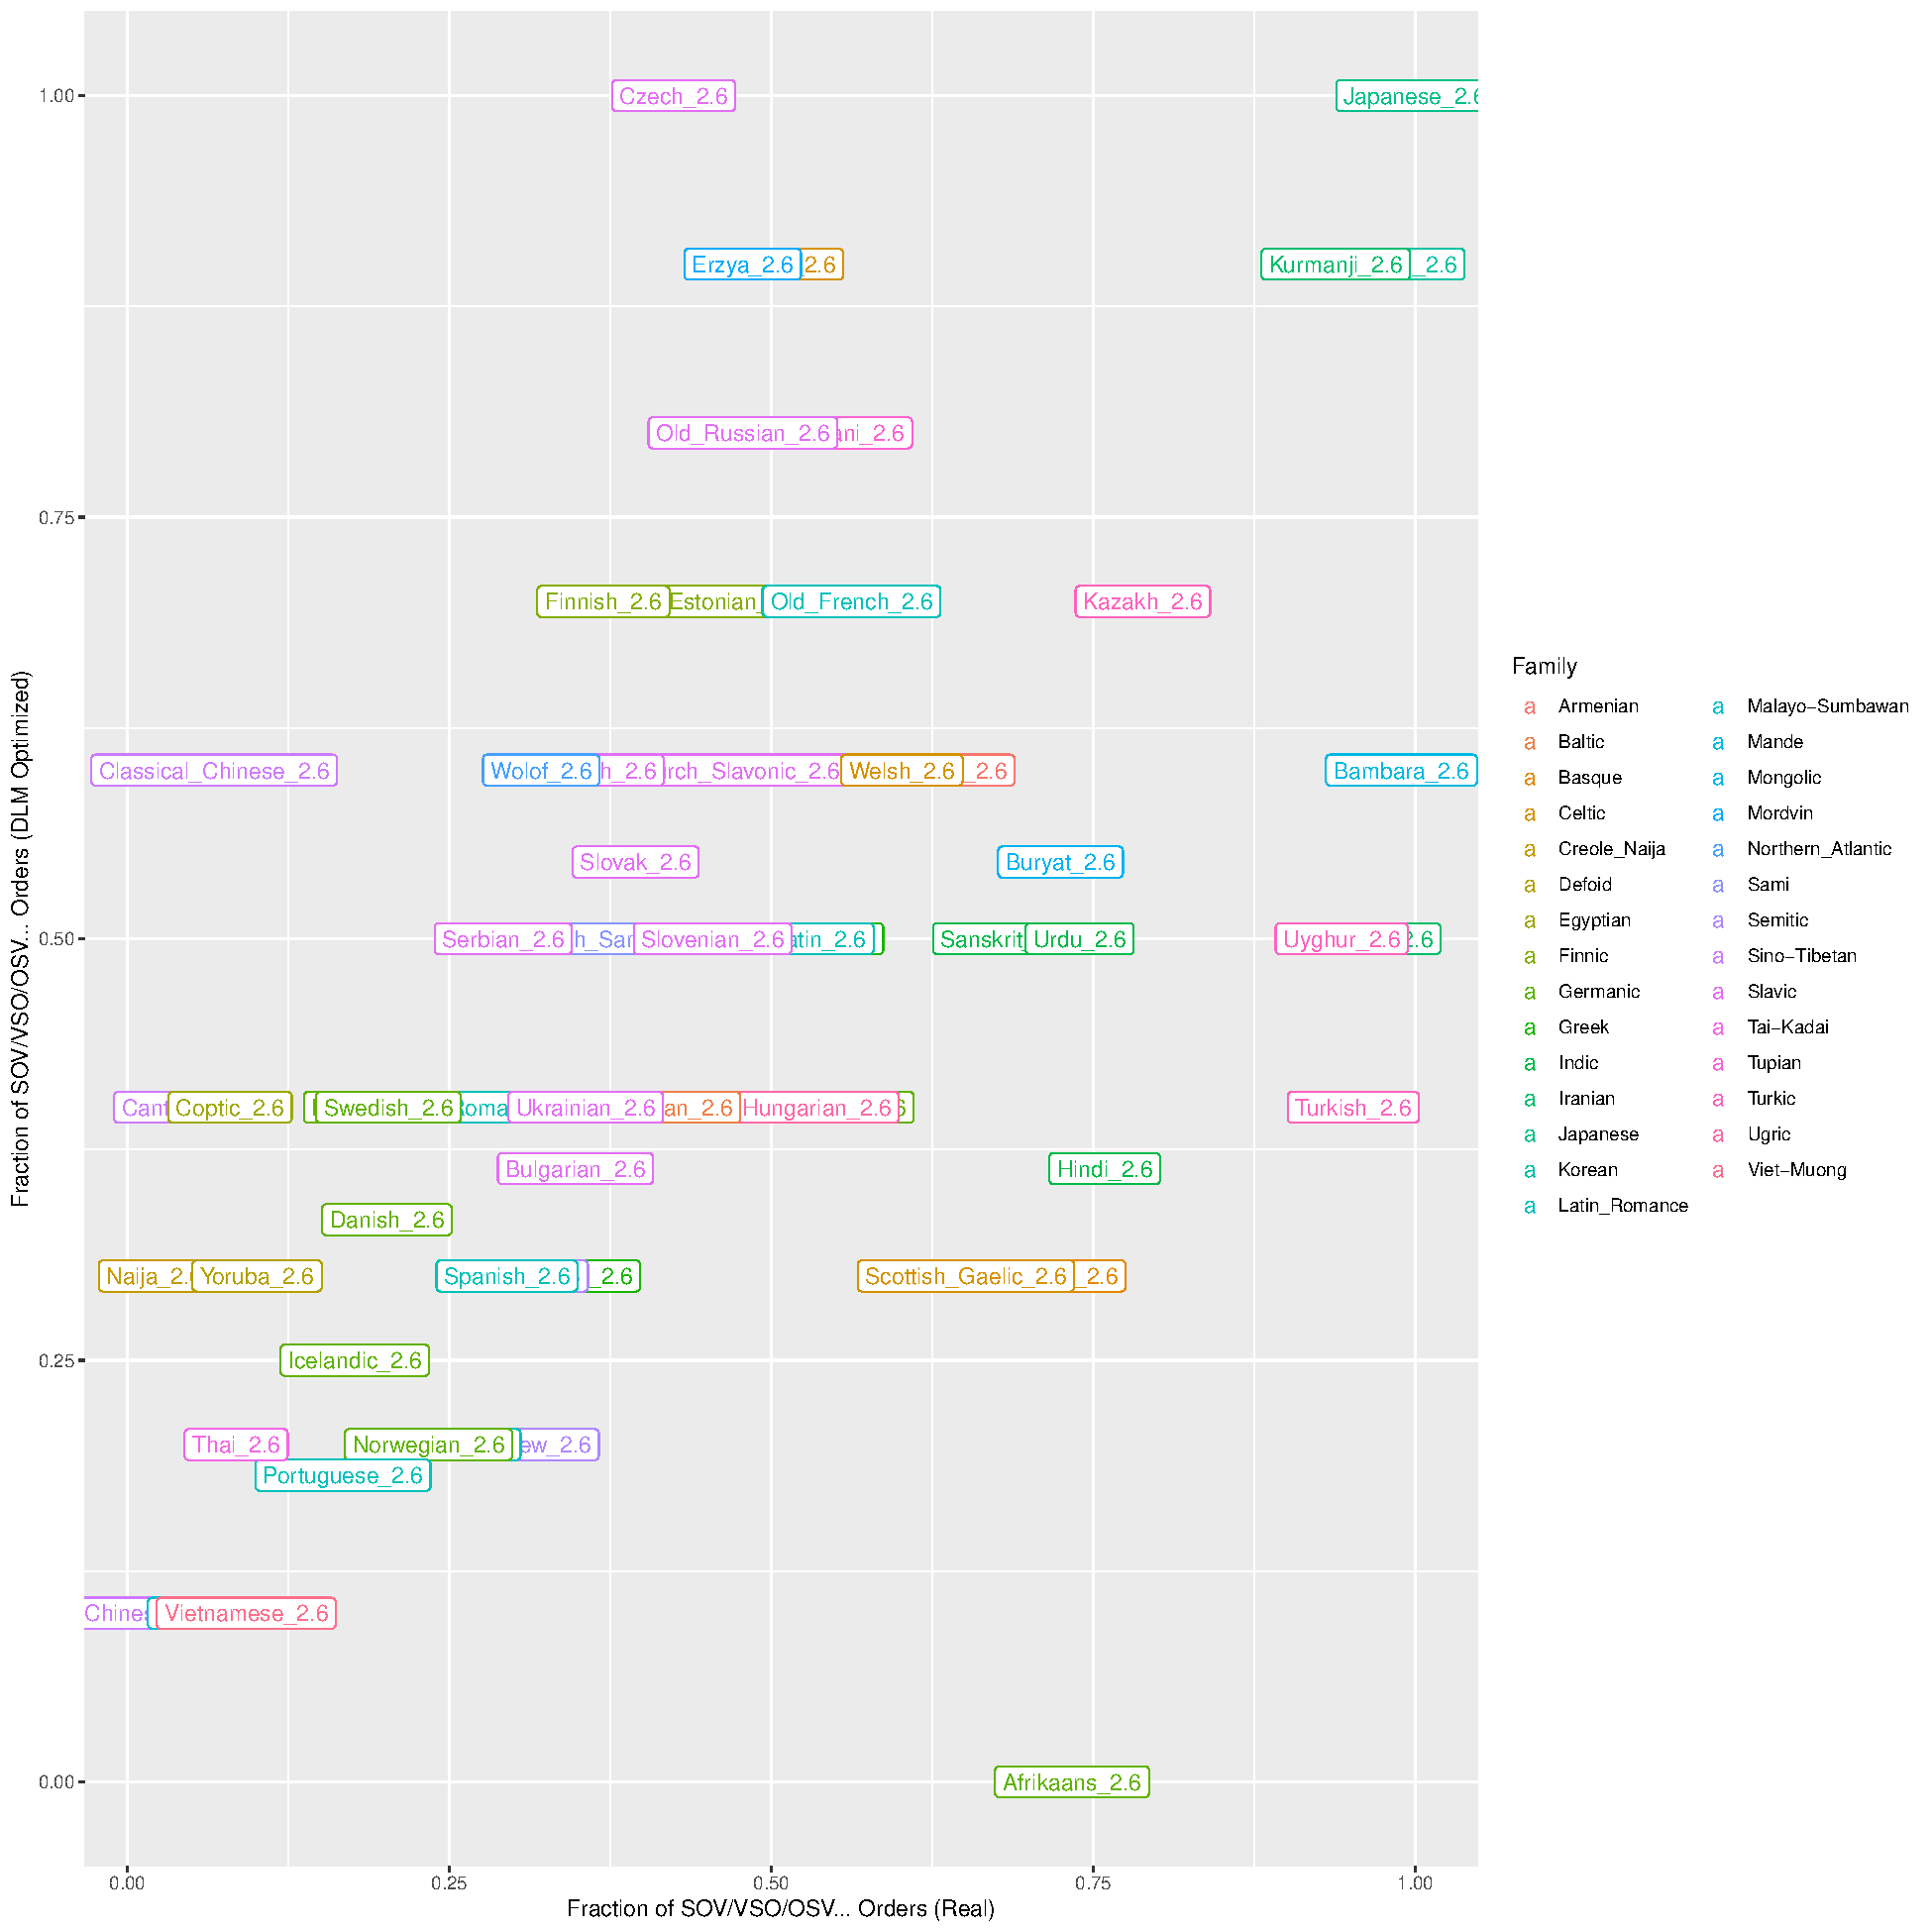
\includegraphics[width=0.95\textwidth]{figures/fracion-optimized_DLM_2.6.pdf}
    \caption{Study 1 (Prevalence of SOV-like order). x-axis real order distributions, y-axis model prediction.}
    \label{fig:study1}
\end{figure}


\begin{figure}
    \centering
    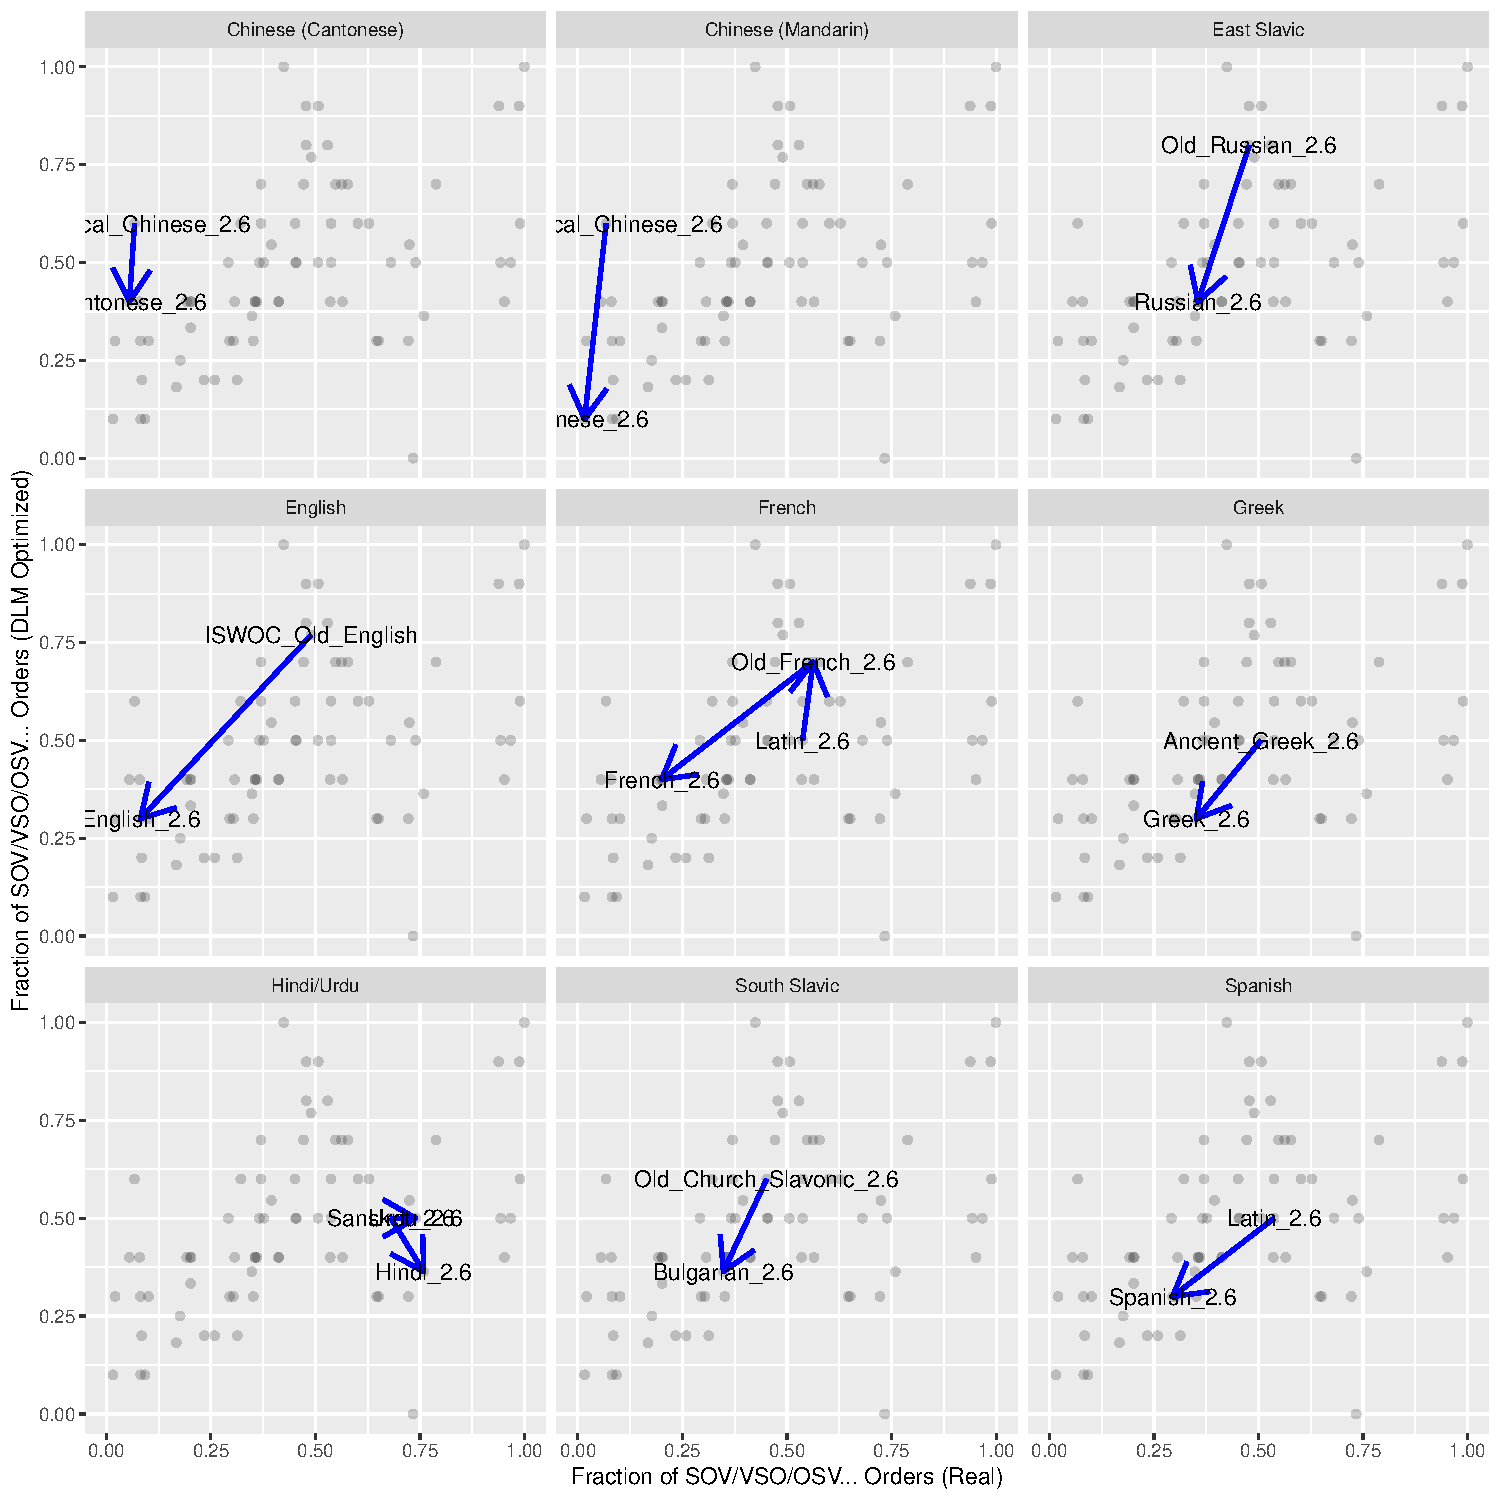
\includegraphics[width=0.95\textwidth]{figures/historical_2.6.pdf}
    \caption{Study 1 (historical changes)}
    \label{fig:historical}
\end{figure}




\section{Study 2: Co-Expressing Subjects and Objects}

-In what ways do usage patterns influence which word order is optimally efficient?

-Co-expression of subjects and objects (referenced from the thought experiment above)

-Results: Figure \ref{fig:study2} plus stats

{\color{blue}Did you mention that there were some novel discoveries or generalizations, do you want to mention them here?}

\begin{figure}
    \centering
    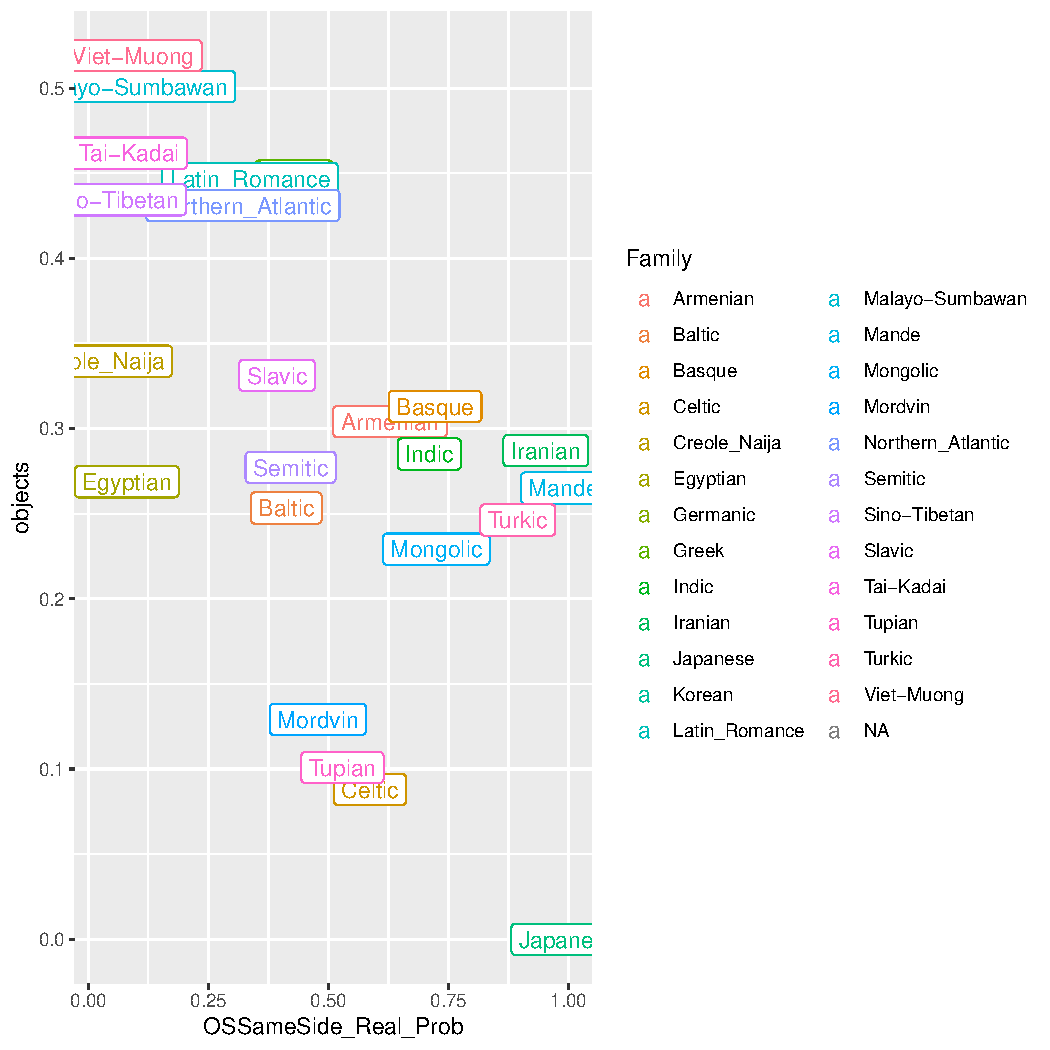
\includegraphics[width=0.95\textwidth]{figures/objects-order-families.pdf}
    \caption{Study 2 (Coexpression of suibjects and objects)}
    \label{fig:study2}
\end{figure}


%\section{Hypotheses}

%SVO preferred when S,O both present, and when O long and S short.

%SOV, VSO orders preferred when O short/not present/intransitive, and when embedded

%Relevant data

%- intransitive subjects behaving like objects

%- Continental West Germanic (except Yiddish). Main clauses predominant SVO/OSV; embedded clauses SOV/OSV.

%- languages with predominant VSO, but alternative SVO in matrix clauses: Standard Arabic, Berber, Ancient Egyptian

%- relative clauses in Bantu: Demuth,Katherine,andCarolynHarford.1999.Verb raising and subject inversion in Bantu relatives. Journal of African Languages and Lingustics20:41ñ61.


\section{Discussion}

{\color{blue} 1. how this work impacts the research on basic word order, and particularly, extends the theory of efficient communication and suggests new functional pressures in shaping the evolution of syntactic structure.}\\

{\color{blue} 2. how this work is limited.} \paragraph{Causal direction} can't decide. not logically necessary that there even is a single causal direction across languages and time.


(There is a linguistic debate on the classification of languages into discrete basic word order types. We sidestep this issue by acknowledging that there is a continuous spectrum).


\section{Conclusion}

\section*{Methods}

{\color{blue}Detailed methods for reproducing this work are typically written in the last section in a NHB article. Include data and code repo and explicit statement that will support replicating all the findings.}\\

{\color{blue}Prepare supplementary material if need be, e.g., you might want to insert a table and map of all languages and their families, dates or periods of time covered, and their word order(s) etc, as well as the detailed experimental parameters.}


\paragraph{Ordering Grammars}


%- flexible

%$a = \sum_i a_{x_i}$

%where $x$ is a feature vector encoding relevant properties of the word. Concretely, we choose the following:
%- dependency label and POS tag
%- dependency label and POS tag and length of the constituent
%- for each sibling, its dependency label + POS tag + length of the constituent

While (CITE) introduced this stochastic parameterization to enable gradient-based optimization, we use it to model word order flexibility.

\paragraph{Creating Optimized Grammars}




\bibliography{literature}
\bibliographystyle{acl_natbib}


\end{document}



